\frame{
\frametitle{Antialiasing}

Algunas líneas en OpenGL especialmente las casi horizontales o verticales con cierto grado de inclinación, parecen irregulares.

Estos bordes dentados aparecen porque la línea ideal se aproxima por una serie de píxeles que deberá situarse en la cuadrícula de píxeles.

Por ejemplo:

        \begin{center}
                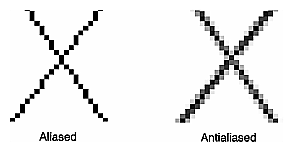
\includegraphics[width=0.6\textwidth]{img/antialiasing}
        \end{center}

}

\frame{
\frametitle{Casos}

Existen varios casos en donde ocurre el fenómeno de aliasing, y para ello también, existen varias técnicas
para realizar antialiasing, como:

\begin{itemize}
	\item Líneas y Puntos Antialiasing
	\item Polígonos Antialiasing
	\item Multisampling
	\item Antialiasing con texturas
	\item Antialiasing with accumulation buffer
\end{itemize}

Para este trabajo se tomaron las primeras dos técnicas para experimentar.
}

\frame{
\frametitle{Antialiasing Línea y puntos}

Debe considerarse por separado de antialiasing polígono ya que las técnicas suelen ser bastante diferente. 
Matemáticamente, una línea es infinitamente delgada. El intento de calcular el porcentaje de un pixel cubierto por un objeto 
infinitamente delgada sería imposible, por lo general, uno de los dos métodos siguientes se utiliza:

\begin{itemize}
	\item La línea se modela como un largo, delgado, de un solo píxel de ancho cuadrilátero. 
		El porcentaje de cobertura de píxel se calcula para cada píxel de la línea y el porcentaje de 
		cobertura se utiliza como el valor alfa de la mezcla.
	\item La línea se modela como un objeto brillante infinitamente delgada y transparente.  
\end{itemize}


}

\frame{
Para realizar este procedimiento en OpenGL, se habilita glEnable pasando GL\_POINT\_SMOOTH o GL\_LINE\_SMOOTH. Además se
puede sugerir una calidad llamando glHint, y se le puede pasar GL\_FASTEST para indicar por ejemplo la opción más eficiente,
o GL\_NICEST para indicar la mejor calidad, o GL\_DONT\_CARE para no elegir nada.

Ejemplo Tomado del redbook.
}

\frame{
\frametitle{Polygon antialiasing}
En el caso de los polígonos, el fenómeno de aliasing ocurre en los bordes o arístas del mismo (dependiendo la forma).

En los bordes de polígonos rellenos es similar a los puntos de suavizado de líneas y líneas. Sin embargo, 
los polígonos anti-aliasing en modo color índice, no es práctico ya que las intersecciones son los objetos más comunes y que 
realmente necesita usar Blending de OpenGL para obtener resultados decentes.

El funcionamiento es similar, se llama glEnable con GL\_POLYGON\_SMOOTH, esto hace que los píxeles en los bordes del polígono sean 
asignados a valores fraccionarios de alfa sobre la base de su cobertura. Tambien se puede proporcionar valores para GL\_POLYGON\_SMOOTH\_HINT.

}
